\chapter{Implementación y pruebas}
Siguiendo con lo definido en el Capítulo \ref{disenio}, donde se han definido los tres bloques que forman el stack MEAN, en este capítulo se procederá a la explicación de su implementación. Para ello, de igual forma al capítulo anterior, se ha hecho una separación de los tres bloques en los que primeramente se expondrá la especificación de las herramientas necesarias para el desarrollo procurando escoger las versiones LTS para seguir durante un número determinado de años recibiendo actualizaciones de soporte. Por supuesto, se describirá el proceso llevado a cabo de programación y, como toda buena implementación, ésta será acompañada de las pruebas que correspondan para corroborar el correcto funcionamiento de la plataforma.

\section{Implementación del servidor y de la base de datos} \label{implementacion-server}
En este apartado se expondrán las herramientas y el procedimiento llevado a cabo para el desarrollo del servidor y el establecimiento de la base de datos utilizada por este. Es destacable mencionar, que previamente se ha hecho una investigación y aprendido Node.js y Express a través de distintos tutoriales y con el libro \textit{''Web development with node and express: leveraging the JavaScript stack''} para tomar las bases de ambas tecnologías \cite{brown2019web}

\subsection{Herramientas para el desarrollo}
Por un lado, para la base de datos se ha utilizado \textbf{MongoDB} haciendo uso del servicio proporcionado en la nube de \textbf{MongoDB Atlas} para la administración de bases de datos MongoDB. En dicho servicio se ha elegido el clúster gratuito con ubicación en París por cercanía, de 512Mb el cual utiliza la versión de MongoDB 5.0.6. 

Por otro lado, para el servidor se han escogido las versiones LTS de \textbf{Node.js} y \textbf{Express} las cuales son 18.12 y 4.18, respectivamente. Por supuesto la utilización de dichas herramientas implica una implementación con el lenguage de programación \textbf{JavaScript}. Además, es muy importante destacar la utilización del administrador de procesos \textbf{PM2} version 5.2 que permite tener dos instancias totalmente iguales del servidor, una activa y otra \textit{''dormida''}, de forma que si la activa falla se despierta a la segunda instancia y se crea una nueva dormida. Por último, para probar las llamadas a la API se ha elegido \textbf{Postman}.

\subsection{Proceso de desarrollo}
Para dar comienzo a la implementación de DayDay se ha creado primeramente la base de datos con nombre ''dd\_db'' junto con las collecciones ya descritas en la Sección \ref{bd}. \bigskip

Con la base de datos ya creada, es momento de crear el servidor y conectarlo a esta. Dadas las colecciones definidas de \textbf{usuarios} y \textbf{citas} se ha hecho una separación de ambas entidades en los \textbf{controladores} de Node.js encargados de toda la lógica de la plataforma, así como los \textbf{modelos} que definen la estructura de los documentos de dichas colecciones. A continuación se precisa la lógica que lleva cada controlador:

\begin{itemize}
    \item \textbf{Controlador de usuarios}: Encargado de toda la lógica CRUD referente a los usuarios. En este controlador se ha de destacar la creación de usuarios, pues los usuarios son creados sin contraseña. Para el establecimiento de ella se le manda al usuario un email de activación de cuenta con un enlace que contiene como parámetro un token JWT previamente generado a partir de una clave secreta almacenada en el fichero \textit{.env} que redirige al usuario al cliente para que pueda establecer su contraseña. Para poder llevar a cabo la emisión de este email se utiliza un módulo de Node.js llamado \textbf{nodemailer} que utiliza como ''host'' Gmail y las credenciales de un correo electrónico creado para la plataforma. Exactamente de igual forma, se procede en la función encargada de enviar el correo para la recuperación de contraseña. Por supuesto, en cada función de este controlador se hace una comprobación previa del rol del usuario para darle o no permiso a realizar la operación, en caso de que éste no lo tuviera se mandaría un código de error 401.
    \item \textbf{Controlador de citas}: Este controlador es el corazón de la plataforma DayDay, en este caso encargado de todas las operaciones CRUD referentes a las citas y en particular hay dos funciones que resultan clave y las cuales hay que resaltar. Para crear una cita asociada a un psicólogo se debe de conocer previamente su disponibilidad, para ello se ha creado una primera función responsable de devolver el rango de horas disponibles para el comienzo de una cita de cinco en cinco minutos. Para lo cual la función recibe el día en el que se quiere realizar la cita y partiendo desde la hora de apertura hasta la hora de cierre de la clínica y habiendo obtenido las citas previamente reservadas se establece que una hora estará disponible teniendo en cuenta que las citas tienen un mínimo de duración de una hora si: 
    \begin{itemize}
        \item No coincide con la hora inicio de otra cita ya reservada.
        \item Desde dicha hora hasta pasada una hora exacta no existe dentro de ese intervalo otra cita.
        \item La hora de después de esa hora no es posterior al cierre de la clínica.
    \end{itemize}  
    Una vez es conocida la hora de inicio deseada para un día y un psicólogo en concreto, la segunda función nos permite conocer los horas disponibles de fin de una cita, pues las citas pueden ser tan extensas como quiera el paciente siempre y cuando no interfiera con la cita de otro. Siguiendo esto, las horas de fin disponibles de una cita serán aquellas que comiencen una hora después de la hora de inicio elegida y estas son incrementadas de cinco en cinco minutos y consideradas disponibles hasta interferir con la hora de inicio de otra cita.
\end{itemize}

Para poder acceder a las funcionalidades dadas por estos controladores y construir un servidor con Node.js se ha utilizado Express, herramienta la cual ha permitido registrar las distintas rutas de la API a las que podrá acceder el cliente (Figura \ref{fig:rutas}): 

\begin{figure}[H]
    \centering{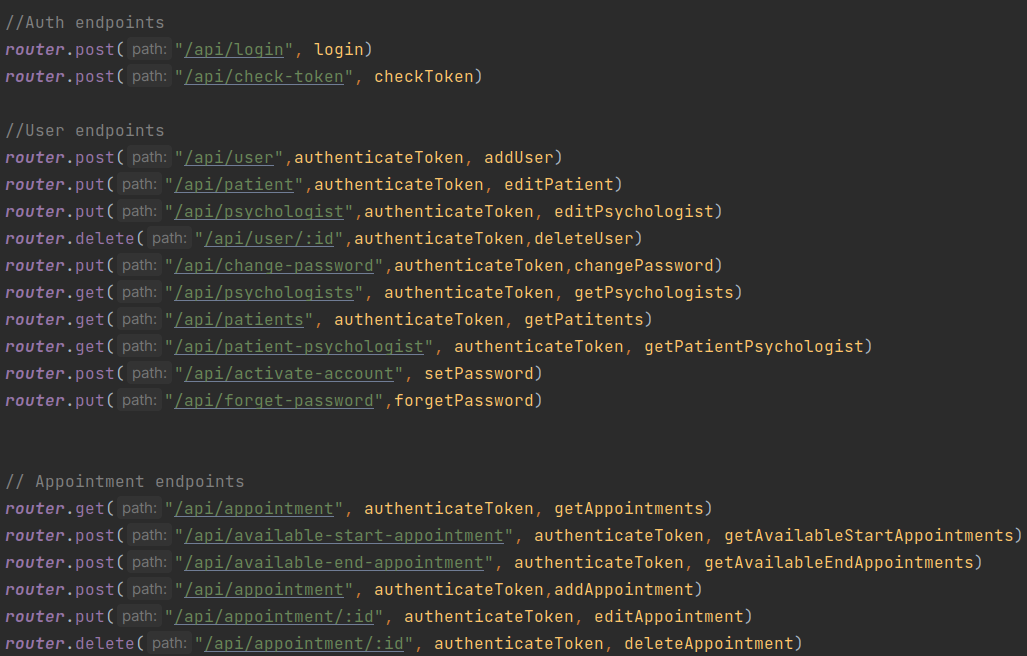
\includegraphics[scale=0.4]{doc/imagenes/rutas.png
    }}
    \caption{Rutas de la API de DayDay}
    \label{fig:rutas}
\end{figure}

De la Figura \ref{fig:rutas} hay que resaltar las funciones \textbf{''login''}, \textbf{''authenticateToken''} y \textbf{''checkToken''}. Estas tres funciones pertenecen a un tercer controlador responsable de la autenticación y autorización en la plataforma. En primer lugar la función ''login'' es la utilizada para el inicio de sesión en la plataforma en la que se chequea si las credenciales son correctas y si lo son se procede a la generación de un token JWT firmado con una clave secreta cuyo ''payload'' es el email del usuario. Una vez generado el JWT se manda como cookie en la respuesta que contiene el email, id, nombre, apellidos y rol del usuario en formato JSON. Resulta muy importante destacar que para tener la mayor seguridad posible en la API siguiendo lo establecido en el artículo \textit{''A Case Study on Cookies and Cyber Security''} \cite{kumawatcase}, las cookies se han establecido como \textbf{''httpOnly''} para que la cookie sólo sea accesible a través de HTTP, \textbf{''sameSite''} para sólo poder enviar la cookie al contexto propio y por último \textbf{''secure''} para que sólo se manden exclusivamente por HTTPS. Para proteger el resto de rutas a las que no puede acceder un usuario que no se haya indentificado en la plataforma se utiliza la función ''authenticateToken'' a modo de middleware para verficar que la cookie enviada en la petición es válida, si lo es se continuará con la petición, en caso contrario se retornará un 401. En cuanto a la función ''checkToken'', esta es llamada en aquellas peticiones en las que se quiera comprobar un token desde el cliente, lo cual se llevará acabo para el acceso a las vistas de activación de cuenta o reestablecimiento de contraseña. \bigskip

En referente a lo que concierne a la gestión y conexión con la base de datos se ha utilizado el módulo \textbf{mongoose} que ha permitido hacer una especificación de los esquemas de las colecciones de citas y usuarios y la conexión con la base de datos encontrada en MongoDB Atlas utilizando la URI proporcionada.

Por último, debido a que el proceso de un servidor Node.js Express deja de funcionar si ocurre un fallo en la API se ha decidido utilizar PM2 para hacer una gestión de ello. Para lo cual, como se ha descrito con anterioridad, se ha creado un archivo \textbf{''.process.js''} que contiene la siguiente configuración para lanzar 2 instancias (Figura \ref{fig:pm2}):

\begin{figure}[H]
    \centering{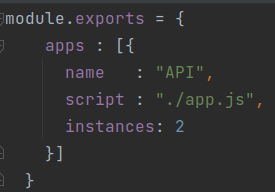
\includegraphics[scale=0.4]{doc/imagenes/pm2.png
    }}
    \caption{Configuración de PM2}
    \label{fig:pm2}
\end{figure}


\section{Implementación del cliente}
Al igual que en el apartado anterior (Sección \ref{implementacion-server}), a continuación se indicarán las herramientas utilizadas en la implementación del cliente así como el proceso llevado a cabo para su programación. 

\subsection{Herramientas para el desarrollo}
Para el desarrollo del cliente de la plataforma se ha utilizado Node.js con su versión LTS 18.12 utilizado para la gestión de módulos y \textbf{Angular} con la versión 14.2 que es la más reciente, aunque no LTS debido a problemas de incompatibilidad con la versión de Node.js. Dentro del framework de Angular utilizaremos las herramientas clásicas en el desarrollo web: 
 \begin{itemize}
     \item \textbf{HTML} para la estructuración de la web.
     \item \textbf{SCSS} el cual es un lenguage de hojas de estilo que utiliza la sintaxis de CSS y hereda las propiedades del metalenguaje de hojas de estilo SaaS permitiendo así la posibilidad ofrecida de declaración de variables en hojas de estilo. 
     \item \textbf{TypeScript} lenguage de programación utilizado en Angular para crear las funciones utilizadas por los componentes web.
 \end{itemize}

Además, se utilizarán las siguientes librerías:
\begin{itemize}
    \item \textbf{Angular Material}, librería de componentes de Angular desarrollada por Google.
    \item \textbf{Angular Flex} para conseguir una interfaz responsiva.
    \item \textbf{RxJS}, librería que sigue el patrón \textbf{Observador} que es un diseño de patrón software en el que a un objeto se le suscriben varios para recibir eventos si su estado cambiase. Esto será de gran utilidad para evitar refrescos cuando algún componente de la vista cambie su estado.
\end{itemize}

En cuanto al componente protagonista, el calendario, se planteó utilizar un componente de Angular ya desarrollado para ahorrar tiempo. Tras hacer una investigación se encontraron algunas opciones, pero la mayoría fueron descartadas ya que eran de pago o por su poco atractiva interfaz. Es por esto que finalmente entre todas ellas destacó el componente Angular Schedule de Syncfusion \footnote{\url{https://ej2.syncfusion.com/angular/documentation/schedule/}}.

\subsection{Proceso de desarrollo}
Ahora que conocemos las herramientas usadas para el desarrollo del cliente, hemos diseñado los mockups en la Sección \ref{mockup-wirefram} y creado la API finalmente es momento de añadir la pieza final a DayDay, el cliente. \bigskip

Para la comunicación con la API, Angular dispone de unas funciones conocidas como \textbf{''servicios''}. Se han creado cuatro, siendo los tres primeros encargados de llamar a las rutas expuestas en la Figura \ref{fig:rutas}:

\begin{itemize}
    \item \textbf{Servicio de citas}
    \item \textbf{Servicio de usuarios}
    \item \textbf{Servicio de autenticación y autorización}
    \item \textbf{Servicio de snackbar}, es un servicio el cual hace uso de un componente de Angular Material que precisa de un servicio para poder funcionar. Es encargado de mostrar una notificación por pantalla cuando fuera requerido
\end{itemize}

En cuanto a los componentes que conforman la vista se distinguen los siguientes:

\begin{itemize}
    \item \textbf{Componentes accesibles por usuarios no identificaciones}:
    \begin{itemize}
        \item \textbf{Login}, vista dedicada al inicio de sesión en la plataforma utilizado el servicio de autenticación y de autorización
        \item \textbf{Recuperación de contraseña}, muestra un formulario para mandar un email de reestablecimiento de contraseña a la dirección de correo electrónico introducida. Para ello hace uso del servicio de usuarios.
        \item \textbf{Página 404}: Si no existe ninguna ruta asociada a la ruta especificada en el navegador es el componente al que el usuario será redirigido por defecto.
    \end{itemize}
    \item \textbf{Componentes accesibles por todos los roles (administrador, psicólogo y paciente)}:
    \begin{itemize}
        \item \textbf{Calendario}: Es el componente más complejo de la plataforma, en él se ha hecho uso del componente \textbf{''Angular Schedule'' de Syncfusion}. Para este proyecto la interfaz del componente ha tenido que ser bastante moldeada para ajustarse a los requisitos impuestos. Para ello, se han alterados las propiedades CSS de las clases definidas en su HTML en los ficheros SCSS y además se han reemplazado los valores de algunas variables del propio componente a través de HTML como se muestra en la Figura \ref{fig:html-calendar}
        \begin{figure}[H]
            \centering{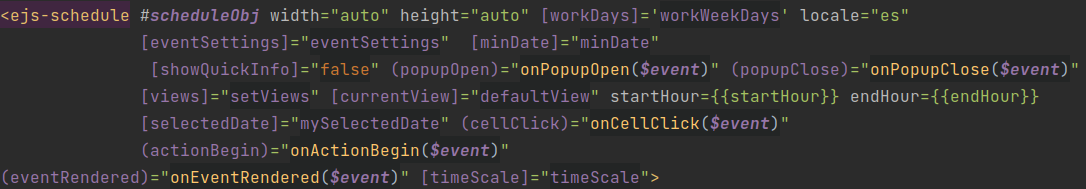
\includegraphics[scale=0.4]{doc/imagenes/html-calendar.png
            }}
            \caption{HTML del componente Schedule de Syncfusion con propiedades modificadas}
            \label{fig:html-calendar}
        \end{figure}
        Para mostrar las citas este componente recibe como fuente de datos un array de JSONs que sigue la estructura del definida en la colección de citas \ref{bd}. En cuanto a la realización de operaciones CRUD con ellas se llama a las funciones \textbf{''onPopupOpen()''} y \textbf{''onPopupClose()''} que reciben como parámetro la información de la celda del calendario a la que se le ha hecho click (hora de inicio de la celda, hora de fin de la celda, fecha y si contiene una cita, toda la información referente a esa cita). Dentro de dichas funciones se lleva a cabo la gestión del formulario que contiene el diálogo emergente para la creación, edición y eliminación de una cita. Dentro de ese diálogo, gracias a RxJS, si el psicólogo seleccionado o la hora de inicio seleccionada cambiaran, las horas disponibles de inicio y fin se verían actualizadas sin refrescar la página. De igual forma es así una vez que se ha creado, añadido o eliminado una cita en el calendario de Syncfusion.
        Este componente hace uso del servicio de citas.
        \item \textbf{Perfil}: Diálogo emergente que muestra la información del usuario actual que se encuentra almacenada en el almacenamiento local del navegador. Además, a través de este componente el usuario puede cambiar su contraseña haciendo uso del servicio de usuarios.
        \item \textbf{Menú lateral}: El menú lateral es visible para todos los roles, sin embargo las opciones mostradas en él son variantes en función de si el rol del usuario tiene permiso o no para acceder a ellas.
    \end{itemize}
    \item \textbf{Componentes accesibles por el administrador}
    \begin{itemize}
        \item \textbf{Lista de pacientes} y \textbf{lista de psicólogos}: Permite la gestión completa de los pacientes y psicólogos. En ambos componentes se abren diálogos emergentes que contienen ''subcomponentes'':
        \begin{itemize}
            \item \textbf{Formulario de creación de pacientes} y \textbf{formulario de creación de psicólogos}
            \item \textbf{Formulario de edición de pacientes} y \textbf{formulario de edición de psicólogos}
            \item \textbf{Formulario de eliminación de pacientes} y \textbf{formulario de eliminación de psicólogos}
        \end{itemize}
        Todos los componentes listados con anterioridad recurren al servicio de usuarios. 
        
        En cuanto a las listas, debido a que se está utilizando el componente \textit{'''mat-table'''} de Angular Material que no permite la actualización de datos sin refresco, la página es recargada cuando se lleva a cabo una operación sobre un paciente. 
    \end{itemize}
    \item \textbf{Componente accesibles con un token válido}
    \begin{itemize}
        \item \textbf{Activación de cuenta}: Vista para que el usuario estableczca una contraseña para su cuenta en la plataforma. Utiliza el servicio de usuarios
        \item \textbf{Reestablecimiento de contraseña}: Vista que permite al usuario establecer una nueva contraseña para su cuenta
    \end{itemize}
\end{itemize}

\subsubsection*{Seguridad}
Tratándose de una plataforma para un centro sanitario, la seguridad en el cliente es crucial. Por ello, se han llevado a cabo una serie de medidas acompañadas a las medidas de seguridad del servidor. \bigskip

Debido a que el servidor es el encargado de hacer las comprobaciones de que el usuario es quien dice ser a través de las cookies, si el cliente recibiera un código 401 la aplicación siempre redireccionará al usuario a la vista de login y tendrá que volver a iniciar sesión para acceder a ella. ¿Cómo se logra esto? A través de los \textbf{interceptores HTTP} de Angular (Figura \ref{fig:interceptor}) responsable de analizar todas las respuestas recibidas al cliente.

\begin{figure}[H]
    \centering{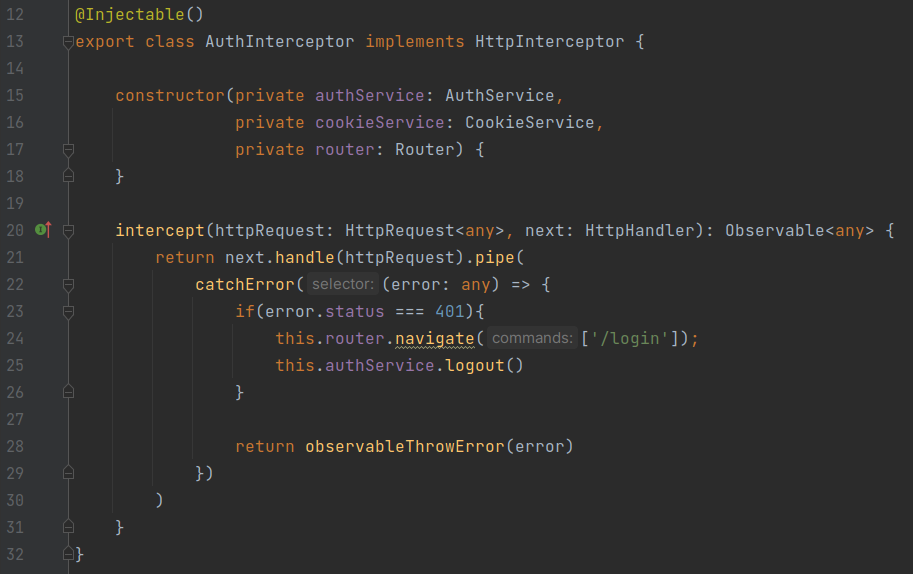
\includegraphics[scale=0.35]{doc/imagenes/interceptor.png
    }}
    \caption{Interceptor HTTP de Angular}
    \label{fig:interceptor}
\end{figure}

En cuanto al acceso restringido a la vistas, se ha creado un \textbf{''Guard''} de Angular (Figura \ref{fig:guard}) el cual obtiene los roles permitidos para la vista a la que se va a navegar y si el rol del usuario identificado no se encuentra entre ellos se le redireccionará a la página 404

\begin{figure}[H]
    \centering{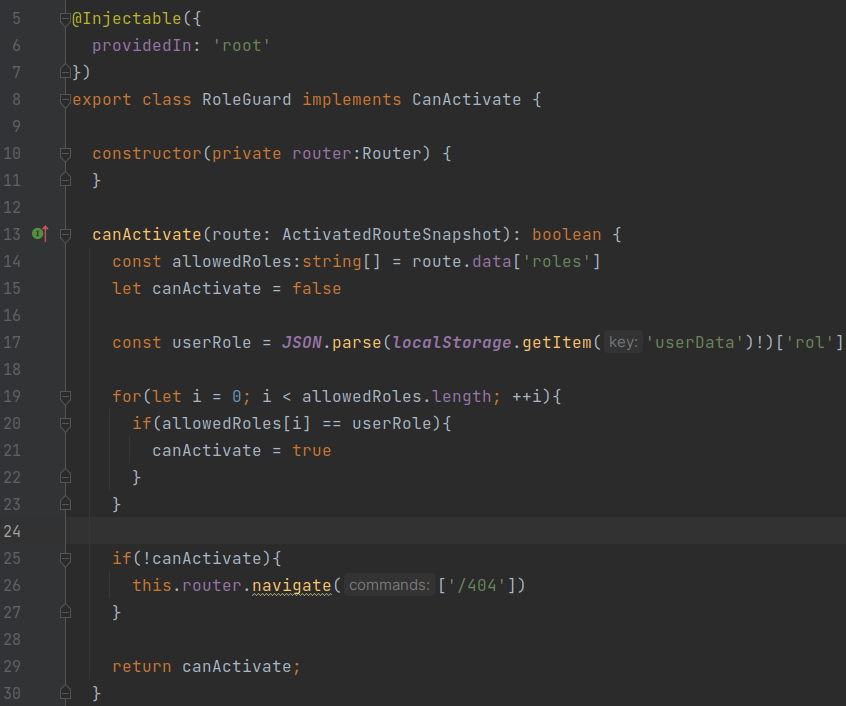
\includegraphics[scale=0.35]{doc/imagenes/guard.png
    }}
    \caption{Role Guard de Angular}
    \label{fig:guard}
\end{figure}

Finalmente, las vistas de activación de cuenta y reestablecimiento de contraseña en las que el usuario sólo posee un token, son sólo accesibles si la función ''\textbf{checkToken()}'' del servidor envía un código 200.

\section{Pruebas}
Son numerosas las posibilidades a elegir para realizar pruebas en Node.js como Jest, Jasmine, AVA o Mocha que son los más populares. Todos ellos son de código abierto, no existen apenas diferencias entre ellos y tras hacer una investigación en la documentación oficial de Node.js en este no se indica en ningún momento qué herramienta es la más conveniente utilizar. Por ello, se han analizado las herramientas nombras en cuanto a uso en la página web ''npm trends'' \footnote{\url{https://npmtrends.com/ava-vs-jasmine-vs-jest-vs-mocha}} y se ha observado (Figura \ref{fig:tests-stats}) que las dos primeras posiciones las ocupan Jest y Mocha:

\begin{figure}[H]
    \centering{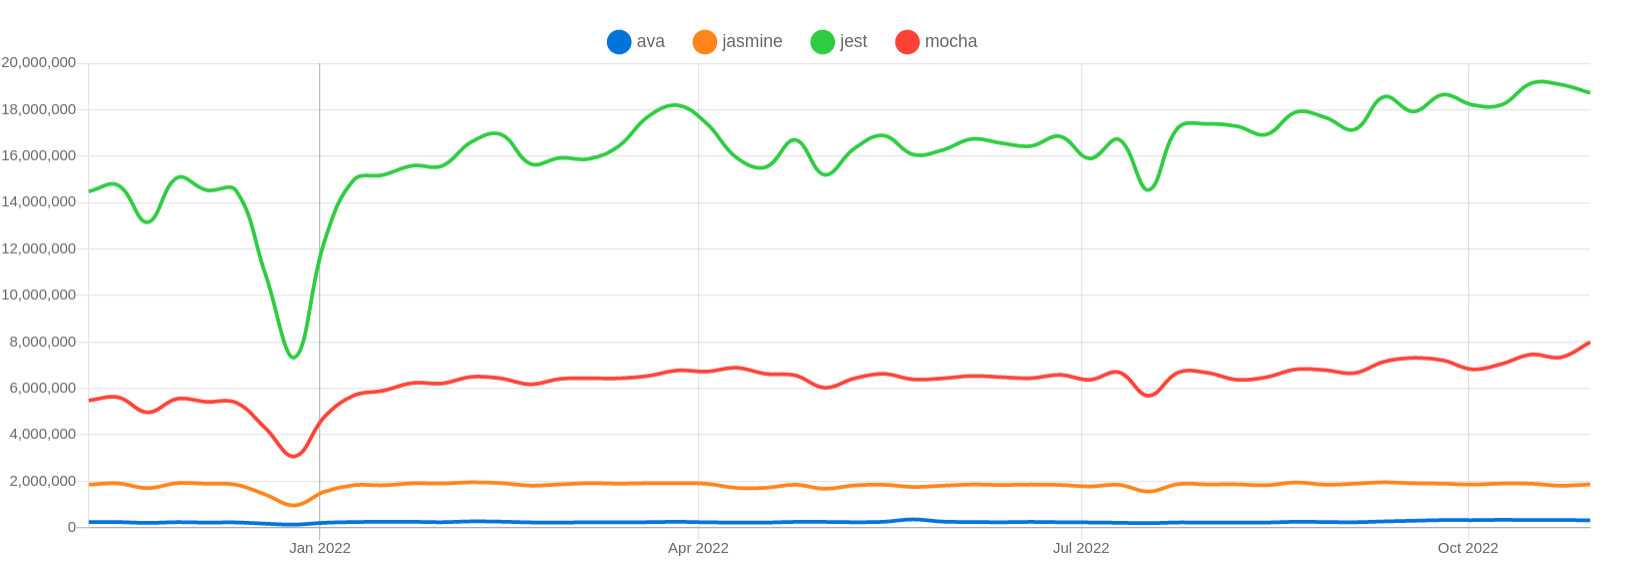
\includegraphics[scale=0.25]{doc/imagenes/test-stats.png
    }}
    \caption{Número de descargas en el último año de Jest, Jasmine, AVA y Mocha}
    \label{fig:tests-stats}
\end{figure}

Tomando esto en cosideración y haciendo un pequeño estudio sobre ambas herramientas, finalmente se decidió utilizar \textbf{Mocha} junto con la librería \textbf{Chai}. La principal razón para tomar esta decisión fue lo que bien afirma Santiago Toscanini et al. en su trabajo titulado ''Fundamentos de entrega continua y tecnologías para pipelines de
desarrollo de software'' \cite{toscanini2022fundamentos}, y es que Mocha es más flexible y configurable que Jest. Aunque Jest es más sencillo en cuanto a configuraciones, éste se encuentra más orientado a las pruebas en frontend. \bigskip

En la realización de pruebas para el backend se han planteado tests para cada uno de los endpoints de la Figura \ref{fig:rutas}:

\begin{itemize}
    \item \textbf{Métodos de los endpoints de autorización y autenticación}:
    \begin{itemize}
        \item \textbf{login()}: Se hace una petición enviando un email y contraseña correctos y se espera un código de estado 200 y la existencia de una cookie en la respuesta.
        \item \textbf{checkToken()}: Con una cookie previamente obtenida se envía el JWT de esta haciendo la petición correspondiente y se espera como respuesta un código 200.
    \end{itemize}
    \item \textbf{Métodos de los endpoints de usuarios} (Para realizar la prueba de todas estos métodos previamente se ha debido de haber iniciado sesión a través del endpoint de ''/api/login''):
    \begin{itemize}
        \item \textbf{addUser(), getPatients() y getPsychologists()}: Se envía una petición con todos los datos de un usuario psicólogo, se espera un código 201 y se listan todos los usuarios con ''getPsychologists()'' se obtiene el último creado y se comprueba que el id del usuario creado y el obtenido coinciden. De igual forma se ha probado la adición de un usuario paciente con el endpoint de ''getPatients()'' pasándole como psicólogo asignado el id del psicólogo creado anteriormente.
        \item \textbf{editPatient() y editPsychologist()}: Se edita el nombre del paciente/psicólogo creado anteriormente, se vuelven a listar los pacientes/psicólogos y se obtiene el editado. Si el nombre editado y el introducido coinciden el test es válido.
        \item \textbf{getPatientPsychologist()}: Con el id del paciente creado anteriormente, se pide al endpoint su psicólogo y si el id que retorna coincide con el id del psicólogo creado anteriormente el test es válido.
        \item \textbf{forgetPassword()}: Se envía una petición con el correo electrónico de uno de los usuarios creados anteriormente y se espera un código 201.
        \item \textbf{setPassword()}: Se envía una petición con el correo electrónico de uno de los usuarios creados anteriormente y se espera un código 201.
        \item \textbf{deleteUser()}: Con los ids obtenidos de los anteriores usuarios creado se llama al endpoint y si se recibe un código 201 el test ha sido pasado con éxito.
    \end{itemize}
    \item \textbf{Métodos de los endpoints de citas}:
    \begin{itemize}
        \item \textbf{getAvailableStartAppointments()}: Para un psicólogo previamente creado se piden las horas disponibles para éste un día en concreto. Si la primera hora disponible son las 10:00 el test es correcto
        \item \textbf{getAvailableEndAppointments()}: Para un psicólogo previamente creado y una hora de inicio de cita seleccionada, si la primera hora disponible es una hora después de la seleccionada el test es correcto
        \item \textbf{addAppointment(), editAppointment(), getAppointments(), deleteAppointment()}: se crea una nueva cita para un psicólogo y paciente previamente creados y para una fecha de inicio y fin de cita seleccionadas. Se espera un código de estado 201 como respuesta, si este test es pasado con éxito se listan las citas y el id de la cita listada tiene que coincidir con la creada. Finalmente se edita la hora de fin de una cita y se vuelve a listar ésta, si coincide la introducida con la cita listada el test ha sido pasado con éxito y la cita es borrada esperándose un código de estado 201.
    \end{itemize}
    
\end{itemize}




